\subsubsection{Higher Level Parameters}

The previous efforts of imitating the original function by varying one or multiple of the parameters $a_L, b_L, c_L, a_R, b_R,$ and $c_R$ did not bring the wanted results.
Therefore new parameters will be created, that are tied directly to characteristics of the function.
\todo{describe parameters better}
For example the parameters $A, B,$ and $C$.
Where $A$ is tied to the value of the function at the left edge of branches $\B$ and $\D$, $f(1) = A$.

\todo{here we have mod 4, describe, explain}

\todo{solve parameters}

\begin{figure}
    \centering
    \includegraphics[width=0.6\textwidth]{40_Quadratic_fittingR/2D_Period_Whole/result.png}
    \caption{2D Scan of Periods of First Fitted Quadratic Model}
    \label{fig:quadratic.full.fit.1.Period}
\end{figure}


\begin{figure}
    \centering
    \begin{subfigure}{0.3\textwidth}
        \centering
        \includegraphics[width=\textwidth]{40_Quadratic_fittingR/Cobweb_A/result.png}
        \caption{At Point A}
        \label{fig:quad.full.fit.1.CobwebA}
    \end{subfigure}
    \begin{subfigure}{0.3\textwidth}
        \centering
        \includegraphics[width=\textwidth]{40_Quadratic_fittingR/Cobweb_B/result.png}
        \caption{At Point B}
        \label{fig:quad.full.fit.1.CobwebB}
    \end{subfigure}
    \begin{subfigure}{0.3\textwidth}
        \centering
        \includegraphics[width=\textwidth]{40_Quadratic_fittingR/Cobweb_C/result.png}
        \caption{At Point C}
        \label{fig:quad.full.fit.1.CobwebC}
    \end{subfigure}
    \caption{Cobwebs at Different Points}
    \label{fig:quad.full.fit.1.Cobwebs}
\end{figure}

The cobwebs show that along these regions of the same period, the symbolic sequence evolves just like the symbolic sequence evolved in the original model along the chains of the same period.
Points of the sequence jump from branches $\A$ and $\C$ to branches $\B$ and $\D$.

\todo{changing the parameters of left branch gives us gecko formation}
Lighter areas indicate the existence of ``type B'' regions.

\begin{figure}
    \centering
    \begin{subfigure}{0.4\textwidth}
        \centering
        \includegraphics[width=\textwidth]{41_Quadratic_fittingR_Gecko/2D_Period_Whole/result.png}
        \caption{Full Model}
        \label{fig:quadratic.full.fit.2.period.full}
    \end{subfigure}
    \begin{subfigure}{0.4\textwidth}
        \centering
        \includegraphics[width=\textwidth]{41_Quadratic_fittingR_Gecko/2D_Period_Whole/result-halved.png}
        \caption{Halved Model}
        \label{fig:quadratic.full.fit.2.period.halved}
    \end{subfigure}
    \caption{2D Scans of Periods of Adjusted Model...}
\end{figure}

\begin{figure}
    \centering
    \begin{subfigure}{0.3\textwidth}
        \centering
        \includegraphics[width=\textwidth]{41_Quadratic_fittingR_Gecko/Cobweb_A/result.png}
        \caption{At Point A}
        \label{fig:quad.full.fit.2.CobwebA}
    \end{subfigure}
    \begin{subfigure}{0.3\textwidth}
        \centering
        \includegraphics[width=\textwidth]{41_Quadratic_fittingR_Gecko/Cobweb_B/result.png}
        \caption{At Point B}
        \label{fig:quad.full.fit.2.CobwebB}
    \end{subfigure}
    \begin{subfigure}{0.3\textwidth}
        \centering
        \includegraphics[width=\textwidth]{41_Quadratic_fittingR_Gecko/Cobweb_C/result.png}
        \caption{At Point C}
        \label{fig:quad.full.fit.2.CobwebC}
    \end{subfigure}
    \caption{Cobwebs at Different Points}
    \label{fig:quad.full.fit.2.Cobwebs}
\end{figure}

\todo{right branch has no local minimum and steepness relatively even => replace w linear branch}

\begin{figure}
    \centering
    \begin{subfigure}{0.4\textwidth}
        \centering
        \includegraphics[width=\textwidth]{50_Quadratic_linearR/2D_Period_Whole/result.png}
        \caption{Full Model}
        \label{fig:quadratic.full.fit.lin.period.full}
    \end{subfigure}
    \begin{subfigure}{0.4\textwidth}
        \centering
        \includegraphics[width=\textwidth]{50_Quadratic_linearR/2D_Period_Whole/result-halved.png}
        \caption{Halved Model}
        \label{fig:quadratic.full.fit.lin.period.halved}
    \end{subfigure}
    \caption{2D Scans of Periods of Adjusted Model...}
\end{figure}

\begin{figure}
    \centering
    \begin{subfigure}{0.3\textwidth}
        \centering
        \includegraphics[width=\textwidth]{50_Quadratic_linearR/Cobweb_A/result.png}
        \caption{At Point A}
        \label{fig:quad.full.fit.lin.CobwebA}
    \end{subfigure}
    \begin{subfigure}{0.3\textwidth}
        \centering
        \includegraphics[width=\textwidth]{50_Quadratic_linearR/Cobweb_B/result.png}
        \caption{At Point B}
        \label{fig:quad.full.fit.lin.CobwebB}
    \end{subfigure}
    \begin{subfigure}{0.3\textwidth}
        \centering
        \includegraphics[width=\textwidth]{50_Quadratic_linearR/Cobweb_C/result.png}
        \caption{At Point C}
        \label{fig:quad.full.fit.lin.CobwebC}
    \end{subfigure}
    \caption{Cobwebs at Different Points}
    \label{fig:quad.full.fit.lin.Cobwebs}
\end{figure}

Scaling the model to the interval $[0, 1]$ and mirroring the influence of the parameter $p_x$ will give the final model.

\todo{how scaled}


\begin{figure}
    \centering
    \begin{subfigure}{0.4\textwidth}
        \centering
        \includegraphics[width=\textwidth]{99_Yunus/2D_Period_Zoomed/result.png}
        \caption{Original Model Full}
        \label{fig:quad.final.comparison.og.full}
    \end{subfigure}
    \begin{subfigure}{0.4\textwidth}
        \centering
        \includegraphics[width=\textwidth]{52_Quadratic_linearR_scaled_mirrored/2D_Period_Whole/result.png}
        \caption{Final Model Full}
        \label{fig:quad.final.comparison.fin.full}
    \end{subfigure} \\
    \begin{subfigure}{0.4\textwidth}
        \centering
        \includegraphics[width=\textwidth]{98_Yunus_modpi/2D_Period_Zoomed/result.png}
        \caption{Original Model Halved}
        \label{fig:quad.final.comparison.og.halved}
    \end{subfigure}
    \begin{subfigure}{0.4\textwidth}
        \centering
        \includegraphics[width=\textwidth]{52_Quadratic_linearR_scaled_mirrored/2D_Period_Whole/result-halved.png}
        \caption{Final Model Halved}
        \label{fig:quad.final.comparison.fin.halved}
    \end{subfigure}
    \caption{Comparison of 2D Scans of Periods of Original and Final Model}
    \label{fig:quad.final.comparison}
\end{figure}
